

\begin{figure*}[h!] 
    \center 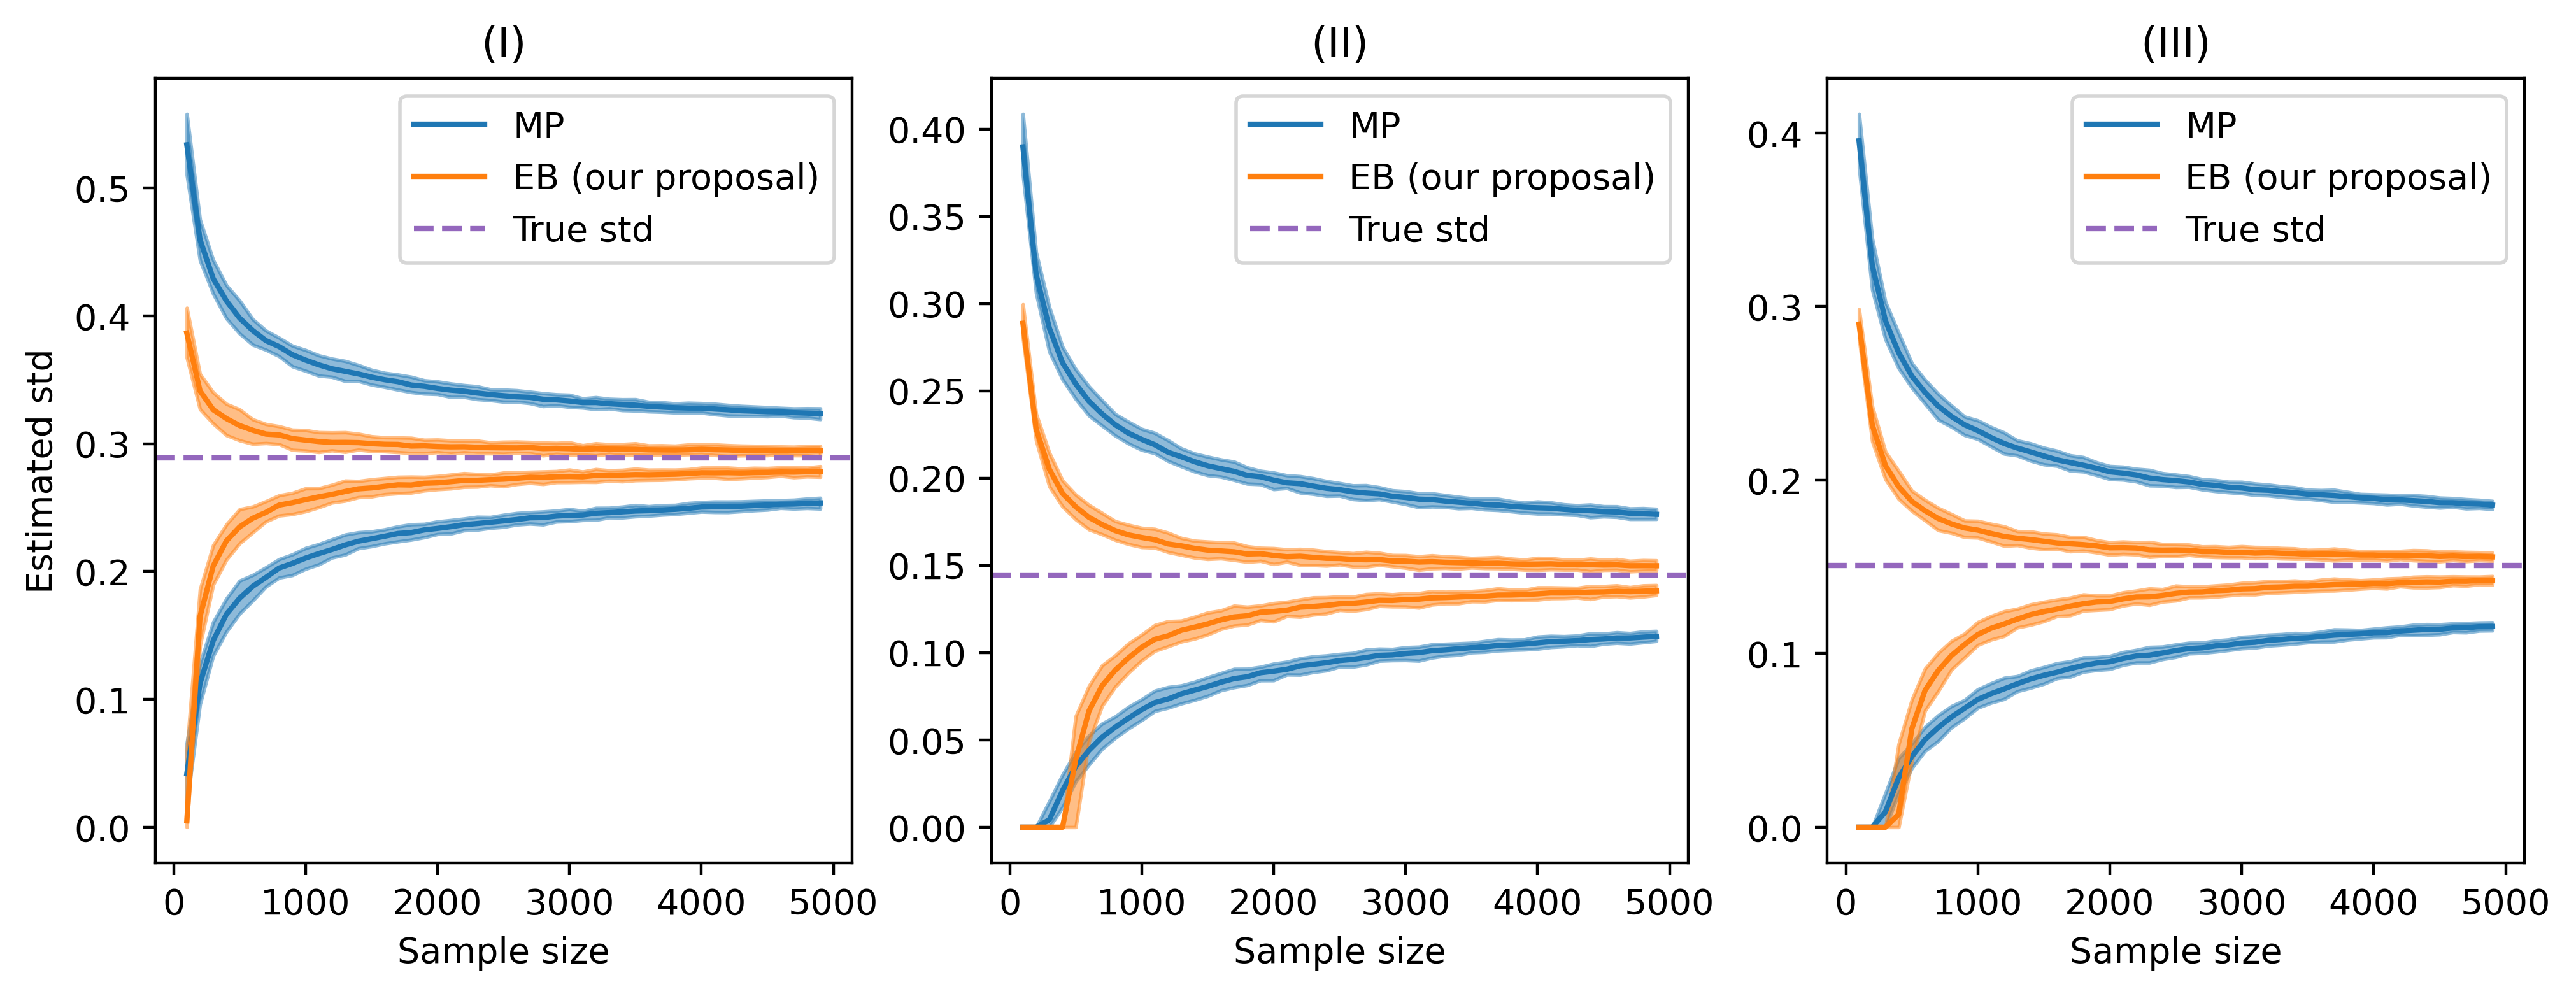
\includegraphics[width=\textwidth]{plots/eb_vs_mp.png}
  \caption{Average confidence intervals over $100$ simulations for the std $\sigma$ for (I) the uniform distribution in $(0,1)$, (II) the beta distribution with parameters $(2, 6)$, and (III) the beta distribution with parameters $(5, 5)$. For each of the inequalities, the $0.95\%$-empirical quantiles are also displayed. The Maurer Pontil (MP) inequality \citep[Theorem 10]{maurer2009empirical} is compared against our proposal (EB). We highlight the improved empirical performance of our methods in all scenarios.} 
  \label{fig:eb_vs_mp}
\end{figure*}


\begin{figure*}[h!] 
    \center 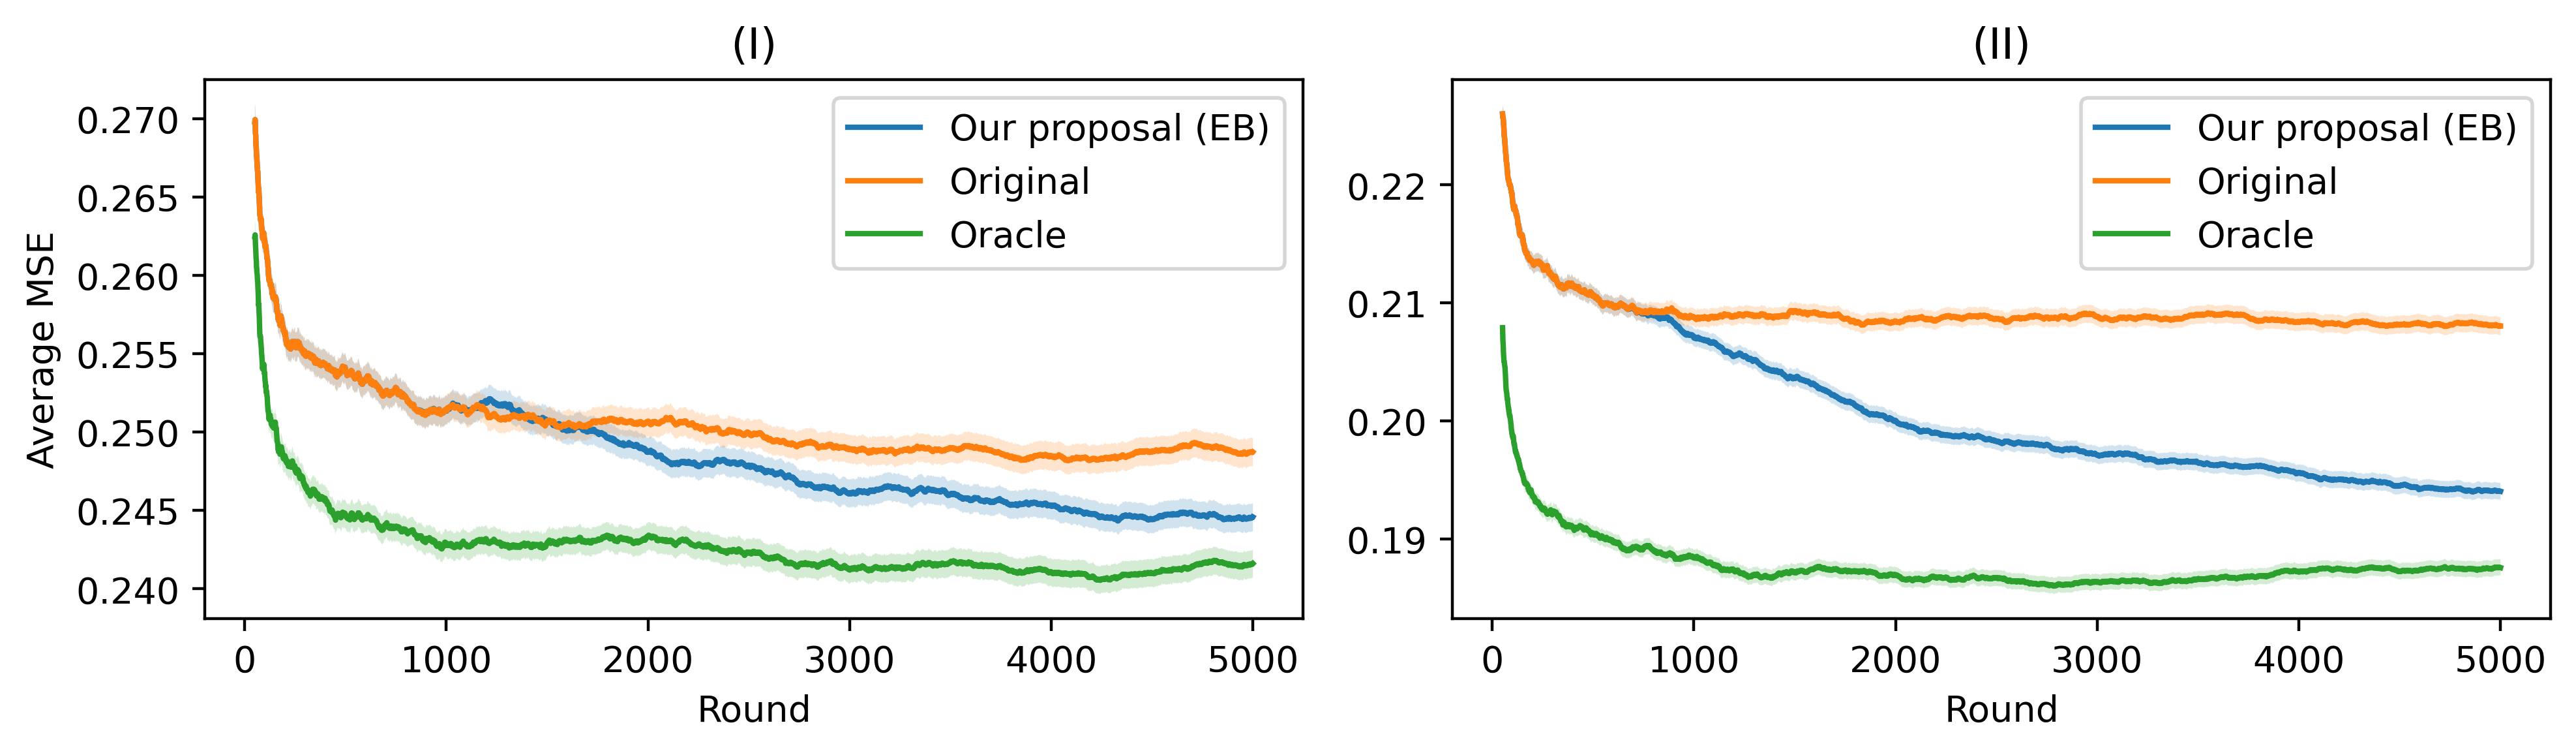
\includegraphics[width=\textwidth]{plots/ojash.png}
  \caption{Mean squared error of the average treatment effect (ATE) sequential estimations, averaged over $1.5e5$ simulations. The placebo and treated potential outcomes are respectively distributed as (I) a $(0,0.7)$-uniform distribution and a $(0,1)$-uniform distribution, and (II) a $(0,1)$-uniform distribution and a $(2, 6)$-beta distribution. The $0.95\%$-empirical quantiles are also displayed. The original algorithm is compared to a variation that replaces their variance confidence sequences with those from Corollary~\ref{corollary:upper_bound}, and an oracle algorithm that has access to the variances is also displayed.} 
  \label{fig:ojash}
\end{figure*}



\section{Experiments} \label{section:experiments}

We devote this section to exploring the empirical performance of both the upper and lower confidence intervals presented in this paper. Note that, in order to obtain confidence intervals for the standard deviation using our approach, it suffices to take the square root of the upper and lower confidence intervals for the variance presented in Section~\ref{section:main_results}.  In all the experiments, we take $\alpha = 0.05$, and the constants $c_1 = \frac{1}{2}$, $c_2 = \frac{1}{2^4}$, $c_3 = \frac{1}{2^2}$, $c_4 = \frac{1}{2}$, $c_5 = 2$.  The code can be found at \href{https://github.com/DMartinezT/emp_bernstein_variance}{https://github.com/DMartinezT/emp\_bernstein\_variance}.  % \href{https://github.com/DMartinezT/empirical_bernstein_variance}{here} The code may be found in the supplementary material. 



\textbf{Batch setting.} We compare our results with 
the inequalities from \citet[Theorem 10]{maurer2009empirical}, which currently constitute the state of the art for the standard deviation, for fixed sample sizes (the more classical batch setting). Figure~\ref{fig:eb_vs_mp} displays the average upper and lower confidence intervals for the standard deviation for different samples sizes for three different bounded distributions. Our inequalities consistently demonstrate improved empirical performance in all evaluated scenarios.  We defer a comparison with other alternatives, such as a double empirical Bernstein inequality on the first and second moment, to Appendix~\ref{section:alternative_approaches}. 




\textbf{Sequential setting.} We explore a direct algorithmic application of our inequalities in the context of optimal adaptive Neyman allocation for randomized control trials (gold standard in causal inference and off-policy evaluation), following the methodology established in \citet{neopane2025optimistic}. In \citet{neopane2025optimistic}, the probability of treatment assignment at a given time is built given the confidence sequences for the standard deviations of the treatment and placebo outcomes. In particular, the treatment policy is sequentially updated, and it requires anytime-valid inference on the variance to prove its optimality. We conduct experiments using the confidence sequences used in \citet{neopane2025optimistic}, %(which are sequential extensions of the results presented in \citet{audibert2006use}),
as well as replacing them with our proposed inequalities, for different potential outcome distributions. We illustrate the results in Figure~\ref{fig:ojash}. Note that our inequalities lead to a substantial improved performance of the adaptive Neyman allocation procedure. Especially in later rounds, our inequalities can lead to performances that are closer to those from an oracle algorithm (that knows the variance) than to those from the original algorithm. 





    

 






